\documentclass[11pt,a4paper]{article}

\usepackage[a4paper,margin=0.75in,right=1in]{geometry}

\usepackage{amsmath,amssymb}
\usepackage{amsthm}
\usepackage{booktabs}
\usepackage{float}
\usepackage{tabularx}
\usepackage{graphicx}
\usepackage{multirow}
\usepackage{mathrsfs}
\usepackage[title]{appendix}
\usepackage{xcolor}
\usepackage{algorithm}
\usepackage{algorithmicx}
\usepackage{algpseudocode}
\usepackage{listings}
\usepackage{subcaption}
\usepackage{tcolorbox}
\usepackage{pgfplots}
\pgfplotsset{compat=1.18}
\usepackage{tikz}
\usetikzlibrary{shapes.geometric, arrows.meta, positioning, calc, fit, backgrounds, shapes.multipart}
\tikzset{
    base/.style = {rectangle, rounded corners, draw=black, align=center, font={\small}, minimum width=6cm, minimum height=1.5cm},
    module/.style = {base, fill=white, minimum width=6cm, minimum height=1.5cm},
    myarrow/.style = {thick, ->}
}
\usepackage[colorlinks=true,linkcolor=blue,citecolor=blue,urlcolor=blue]{hyperref}

\setlength{\belowrulesep}{0pt}
\setlength{\aboverulesep}{0pt}
\setlength{\intextsep}{8pt plus 2pt minus 2pt}

\theoremstyle{plain}
\newtheorem{theorem}{Theorem}
\newtheorem{proposition}[theorem]{Proposition}
\newtheorem{lemma}[theorem]{Lemma}
\newtheorem{corollary}[theorem]{Corollary}
\theoremstyle{definition}
\newtheorem{example}{Example}
\newtheorem{definition}{Definition}
\theoremstyle{remark}
\newtheorem{remark}{Remark}
\renewcommand{\qedsymbol}{$\blacksquare$}

\raggedbottom

\title{Sample Document: A Formatting Template}
\author{Author One, Author Two, and Author Three}
\date{}

\begin{document}
\maketitle

\section{Introduction}

\subsection{Background of the Study}
Placeholder paragraph text. Citations look like this: shortest paths \cite{dijkstra1959note}, or several at once \cite{cormen2009introduction, knuth1997art}. New terms can be set in \textbf{bold}.
\subsection{Statement of the Problem}
Numbered items use \texttt{enumerate}:
\begin{enumerate}
    \item First item, with inline math such as $O(n \log n)$.
    \item Second item.
\end{enumerate}
\subsection{Objectives of the Study}
Placeholder paragraph text introducing the objectives. This study aims to achieve the following:

\begin{enumerate}
    \item First objective, with inline math such as $O(n \log n)$.
    \item Second objective, with a citation \cite{dijkstra1959note}.
    \item Third objective.
\end{enumerate}
\subsection{Definition of Terms}
\begin{description}
    \item[Graph.] A set of vertices together with a set of edges joining pairs of vertices.
    \item[Weight ($w$).] A number attached to an edge, such as a distance.
\end{description}


\section{Review of Related Literature}

\subsection{Example Subsection}
Short prose with grouped citations \cite{dijkstra1959note, cormen2009introduction}. Summary tables use one pattern throughout:

\begin{table}[H]
\centering
\caption{Sample literature summary table.}\label{tab:rrl}
\vspace{4pt}
\begin{tabularx}{\textwidth}{l X X}
\toprule
\textbf{Source} & \textbf{Contribution} & \textbf{Limitation}\\
\midrule
Dijkstra \cite{dijkstra1959note} & Shortest paths with non-negative weights & Fails on negative weights\\
Cormen et al. \cite{cormen2009introduction} & Broad textbook coverage of algorithms & General, not specialized\\
\bottomrule
\end{tabularx}
\end{table}

Cross-references are blue: Table~\ref{tab:rrl}, Section~\ref{sec:model}.

\section{Methodology}

\subsection{Model}\label{sec:model}
\begin{definition}[Weighted graph]\label{def:graph}
A weighted graph is a triple $G=(V,E,w)$ with $w:E\to\mathbb{R}_{\ge 0}$.
\end{definition}
\begin{figure}[H]
\centering
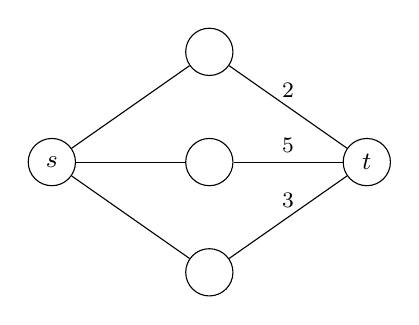
\begin{tikzpicture}[v/.style={circle,draw,minimum size=6mm,inner sep=0pt,font=\small}]
  \node[v] (s) at (0,0) {$s$};
  \node[v] (t) at (4,0) {$t$};
  \foreach \y/\i/\w in {1.4/1/2,0/2/5,-1.4/3/3}{
     \node[v] (m\i) at (2,\y) {};
     \draw (s)--(m\i); \draw (m\i)--node[above,font=\footnotesize]{\w}(t);
  }
\end{tikzpicture}
\caption{A small weighted graph with three routes from $s$ to $t$.}\label{fig:graph}
\end{figure}
A numbered equation and a two-line aligned one:
\begin{equation}\label{eq:path}
  d(s,t) \;=\; \min_{P}\ \sum_{e\in P} w(e)
\end{equation}
\begin{align}
  T_{\text{merge}}(n) &= 2\,T_{\text{merge}}(n/2) + n, \label{eq:merge}\\
  T_{\text{merge}}(n) &= O(n\log n). \nonumber
\end{align}

\subsection{Theory}
\begin{lemma}[Triangle inequality]\label{lem:tri}
For any vertices $a,b,c$, $d(a,c)\le d(a,b)+d(b,c)$.
\end{lemma}
\begin{proof}
Joining a shortest $a$--$b$ path to a shortest $b$--$c$ path gives an $a$--$c$ walk of length $d(a,b)+d(b,c)$. The shortest $a$--$c$ path is no longer than that walk.
\end{proof}
\begin{theorem}[Sum of integers]\label{thm:sum}
For every $n\ge 1$, $\displaystyle\sum_{i=1}^{n} i=\frac{n(n+1)}{2}$.
\end{theorem}
\begin{proof}
By induction. For $n=1$ both sides equal $1$. If it holds for $n$, then $\sum_{i=1}^{n+1} i=\frac{n(n+1)}{2}+(n+1)=\frac{(n+1)(n+2)}{2}$.
\end{proof}
\begin{corollary}
The sum of the first $100$ integers is $5050$, by Theorem~\ref{thm:sum}.
\end{corollary}

\subsection{Verification}
\begin{table}[H]
\centering
\caption{Sample results table.}
\vspace{4pt}
\begin{tabularx}{\textwidth}{c c c X}
\toprule
$n$ & \textbf{Predicted} & \textbf{Measured} & \textbf{Agrees?}\\
\midrule
10 & 55 & 55 & Yes\\
100 & 5050 & 5050 & Yes\\
\bottomrule
\end{tabularx}
\end{table}

\subsection{Pipeline}
\begin{figure}[H]
\centering
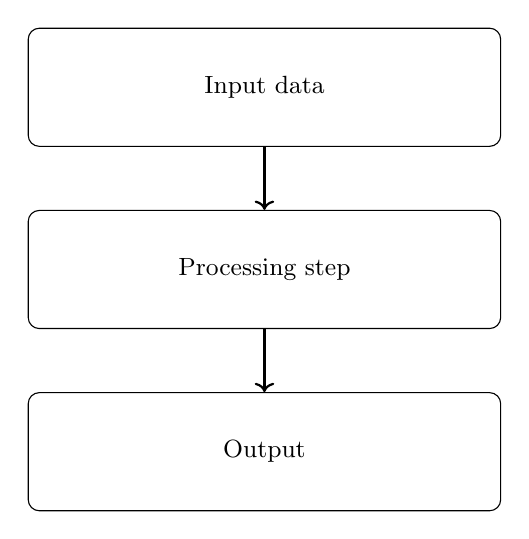
\begin{tikzpicture}[node distance=0.8cm]
  \node[module] (a) {Input data};
  \node[module, below=of a] (b) {Processing step};
  \node[module, below=of b] (c) {Output};
  \draw[myarrow] (a)--(b); \draw[myarrow] (b)--(c);
\end{tikzpicture}
\caption{Flow diagram using the \texttt{module} and \texttt{myarrow} styles.}
\end{figure}

\subsection{Algorithm}
\begin{algorithm}[H]
\caption{Breadth-first search}\label{alg:bfs}
\begin{algorithmic}[1]
\Require Graph $G$, start vertex $s$
\State Mark $s$ visited and add it to queue $Q$
\While{$Q$ is not empty}
  \State $u \gets$ remove the front of $Q$
  \For{each neighbor $v$ of $u$}
    \If{$v$ is not visited} \State mark $v$ visited and add it to $Q$ \EndIf
  \EndFor
\EndWhile
\end{algorithmic}
\end{algorithm}

\subsection{Experiments}
Test cases are run in this order:
\begin{enumerate}
    \item Small hand-made graphs
    \item Randomly generated graphs
\end{enumerate}
\begin{figure}[H]
\centering
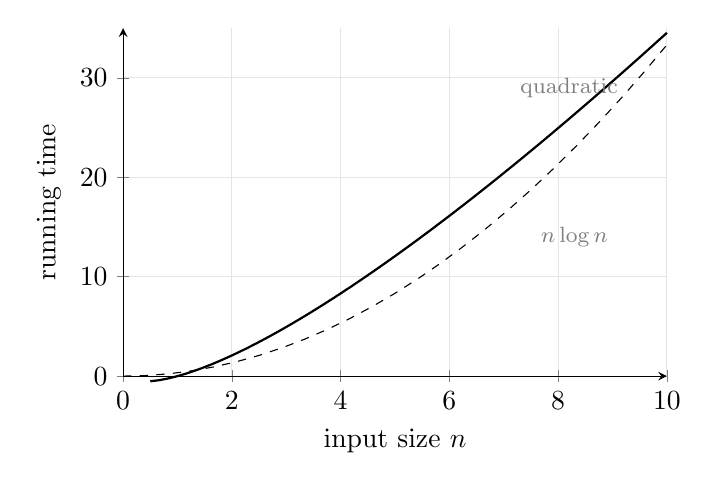
\begin{tikzpicture}
\begin{axis}[width=0.7\textwidth,height=6cm,xlabel={input size $n$},ylabel={running time},
  xmin=0,xmax=10,ymin=0,ymax=35,axis x line=bottom,axis y line=left,clip=false,grid=major,grid style={gray!20}]
  \addplot[domain=0.5:10,samples=60,thick]{x*ln(x)*1.5};
  \addplot[domain=0:10,dashed]{x^2/3};
  \node[font=\footnotesize,gray] at (axis cs:8.2,29) {quadratic};
  \node[font=\footnotesize,gray] at (axis cs:8.3,14) {$n\log n$};
\end{axis}
\end{tikzpicture}
\caption{Growth of two running-time curves (pgfplots).}
\end{figure}
\begin{figure}[H]
\centering
\begin{subfigure}[t]{0.45\textwidth}\centering
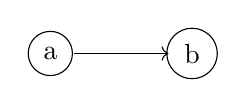
\begin{tikzpicture}\node[draw,circle]{a};\draw[->](0.3,0)--(1.5,0);\node[draw,circle] at (1.8,0){b};\end{tikzpicture}
\caption{First panel.}
\end{subfigure}\hfill
\begin{subfigure}[t]{0.45\textwidth}\centering
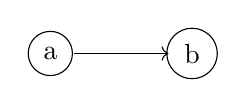
\begin{tikzpicture}\node[draw,circle]{a};\draw[->](0.3,0)--(1.5,0);\node[draw,circle] at (1.8,0){b};\end{tikzpicture}
\caption{Second panel.}
\end{subfigure}
\caption{Side-by-side subfigures.}
\end{figure}

\subsection{Metrics}
Results are reported as in Equation~\eqref{eq:path} and Equation~\eqref{eq:merge}.



\bibliographystyle{plain}
\bibliography{thesis-refs}
\end{document}